\documentclass[twoside]{book}

% Packages required by doxygen
\usepackage{fixltx2e}
\usepackage{calc}
\usepackage{doxygen}
\usepackage{graphicx}
\usepackage[utf8]{inputenc}
\usepackage{makeidx}
\usepackage{multicol}
\usepackage{multirow}
\PassOptionsToPackage{warn}{textcomp}
\usepackage{textcomp}
\usepackage[nointegrals]{wasysym}
\usepackage[table]{xcolor}

% Font selection
\usepackage[T1]{fontenc}
\usepackage{mathptmx}
\usepackage[scaled=.90]{helvet}
\usepackage{courier}
\usepackage{amssymb}
\usepackage{sectsty}
\renewcommand{\familydefault}{\sfdefault}
\allsectionsfont{%
  \fontseries{bc}\selectfont%
  \color{darkgray}%
}
\renewcommand{\DoxyLabelFont}{%
  \fontseries{bc}\selectfont%
  \color{darkgray}%
}
\newcommand{\+}{\discretionary{\mbox{\scriptsize$\hookleftarrow$}}{}{}}

% Page & text layout
\usepackage{geometry}
\geometry{%
  a4paper,%
  top=2.5cm,%
  bottom=2.5cm,%
  left=2.5cm,%
  right=2.5cm%
}
\tolerance=750
\hfuzz=15pt
\hbadness=750
\setlength{\emergencystretch}{15pt}
\setlength{\parindent}{0cm}
\setlength{\parskip}{0.2cm}
\makeatletter
\renewcommand{\paragraph}{%
  \@startsection{paragraph}{4}{0ex}{-1.0ex}{1.0ex}{%
    \normalfont\normalsize\bfseries\SS@parafont%
  }%
}
\renewcommand{\subparagraph}{%
  \@startsection{subparagraph}{5}{0ex}{-1.0ex}{1.0ex}{%
    \normalfont\normalsize\bfseries\SS@subparafont%
  }%
}
\newcommand{\HRule}{\rule{\linewidth}{0.5mm}}
\makeatother

% Headers & footers
\usepackage{fancyhdr}
\pagestyle{fancyplain}
\fancyhead[LE]{\fancyplain{}{\bfseries\thepage}}
\fancyhead[CE]{\fancyplain{}{}}
\fancyhead[RE]{\fancyplain{}{\bfseries\leftmark}}
\fancyhead[LO]{\fancyplain{}{\bfseries\rightmark}}
\fancyhead[CO]{\fancyplain{}{}}
\fancyhead[RO]{\fancyplain{}{\bfseries\thepage}}
\fancyfoot[LE]{\fancyplain{}{}}
\fancyfoot[CE]{\fancyplain{}{}}
\fancyfoot[RE]{\fancyplain{}{\bfseries\scriptsize Generated on Thu Sep 11 2014 23\+:57\+:39 for Reverse Polish Calculator by Doxygen }}
\fancyfoot[LO]{\fancyplain{}{\bfseries\scriptsize Generated on Thu Sep 11 2014 23\+:57\+:39 for Reverse Polish Calculator by Doxygen }}
\fancyfoot[CO]{\fancyplain{}{}}
\fancyfoot[RO]{\fancyplain{}{}}
\renewcommand{\footrulewidth}{0.4pt}
\renewcommand{\chaptermark}[1]{%
  \markboth{#1}{}%
}
\renewcommand{\sectionmark}[1]{%
  \markright{\thesection\ #1}%
}


% Indices & bibliography
\usepackage{natbib}
\usepackage[titles]{tocloft}
\setcounter{tocdepth}{3}
\setcounter{secnumdepth}{5}
\makeindex

% Hyperlinks (required, but should be loaded last)
\usepackage{ifpdf}
\ifpdf
  \usepackage[pdftex,pagebackref=true]{hyperref}
\else
  \usepackage[ps2pdf,pagebackref=true]{hyperref}
\fi
\hypersetup{%
  colorlinks=true,%
  linkcolor=blue,%
  citecolor=blue,%
  unicode%
}

% Custom commands
\newcommand{\clearemptydoublepage}{%
  \newpage{\pagestyle{empty}\cleardoublepage}%
}


%===== C O N T E N T S =====

\begin{document}

% Titlepage & ToC
\hypersetup{pageanchor=false,
             bookmarks=true,
             bookmarksnumbered=true,
             pdfencoding=unicode
            }
\pagenumbering{roman}
\begin{titlepage}
\vspace*{7cm}
\begin{center}%
\textsc{\LARGE IT University of Copenhagen}\\[1.5cm]

\textsc{\Large BDSA 2014 }\\[0.5cm]

% Title
\HRule \\[0.4cm]
{ \huge \bfseries InheritanceRPC Documentation \\ [0.1cm]
    %\large \\ [0.4cm] 
    }

\HRule \\[1cm]
\textsc{\Large Assignment 38 }\\[1.5cm]

% Author and supervisor
\begin{minipage}{1\textwidth}
\begin{center} \large
Anders Wind Steffensen - awis@itu.dk\\
Christopher Blundell - cnbl@itu.dk\\
Pierre Mandas - ppma@itu.dk\\
\end{center}
\end{minipage}
\vfill
{\large Generated by Doxygen 1.8.8}\\
\vspace*{0.5cm}
{\small Fri Sep 19 2014 22:00}\\
\end{center}
\end{titlepage}
\clearemptydoublepage
\tableofcontents
\clearemptydoublepage
\pagenumbering{arabic}
\hypersetup{pageanchor=true}

%--- Begin generated contents ---
\chapter{Namespace Index}
\section{Packages}
Here are the packages with brief descriptions (if available)\+:\begin{DoxyCompactList}
\item\contentsline{section}{\hyperlink{namespace_reverse_polish_calculator}{Reverse\+Polish\+Calculator} }{\pageref{namespace_reverse_polish_calculator}}{}
\end{DoxyCompactList}

\chapter{Hierarchical Index}
\section{Class Hierarchy}
This inheritance list is sorted roughly, but not completely, alphabetically\+:\begin{DoxyCompactList}
\item \contentsline{section}{Inheritance\+R\+P\+C\+\_\+\+Project.\+Inheritance\+R\+P\+C}{\pageref{class_inheritance_r_p_c___project_1_1_inheritance_r_p_c}}{}
\item \contentsline{section}{Inheritance\+R\+P\+C\+\_\+\+Project.\+Inheritance\+R\+P\+Ctests}{\pageref{class_inheritance_r_p_c___project_1_1_inheritance_r_p_ctests}}{}
\item \contentsline{section}{Inheritance\+R\+P\+C\+\_\+\+Project.\+I\+Operation}{\pageref{interface_inheritance_r_p_c___project_1_1_i_operation}}{}
\begin{DoxyCompactList}
\item \contentsline{section}{Inheritance\+R\+P\+C\+\_\+\+Project.\+Binary\+Operation}{\pageref{class_inheritance_r_p_c___project_1_1_binary_operation}}{}
\item \contentsline{section}{Inheritance\+R\+P\+C\+\_\+\+Project.\+Unary\+Operation}{\pageref{class_inheritance_r_p_c___project_1_1_unary_operation}}{}
\end{DoxyCompactList}
\end{DoxyCompactList}

\chapter{Class Index}
\section{Class List}
Here are the classes, structs, unions and interfaces with brief descriptions\+:\begin{DoxyCompactList}
\item\contentsline{section}{\hyperlink{class_calendar_system_1_1_model_1_1_calendar}{Calendar\+System.\+Model.\+Calendar} \\*A class containing a datastructure with I\+Events and provides methods to get the events from the datastructure. }{\pageref{class_calendar_system_1_1_model_1_1_calendar}}{}
\item\contentsline{section}{\hyperlink{class_calendar_system_1_1_view_1_1_calendar_view}{Calendar\+System.\+View.\+Calendar\+View} \\*The calendar view visually represents the calendar of events in the storage }{\pageref{class_calendar_system_1_1_view_1_1_calendar_view}}{}
\item\contentsline{section}{\hyperlink{class_class1}{Class1} }{\pageref{class_class1}}{}
\item\contentsline{section}{\hyperlink{class_calendar_system_1_1_data_storage_1_1_database_storage}{Calendar\+System.\+Data\+Storage.\+Database\+Storage} \\*A storage class which implements the \hyperlink{interface_calendar_system_1_1_data_storage_1_1_i_storage}{I\+Storage} interface. The class is meant to have a connection to a database where events will be added when they are created and put in the local Calendar class. }{\pageref{class_calendar_system_1_1_data_storage_1_1_database_storage}}{}
\item\contentsline{section}{\hyperlink{class_calendar_system_1_1_model_1_1_event}{Calendar\+System.\+Model.\+Event} \\*The event class implements the \hyperlink{interface_calendar_system_1_1_model_1_1_i_event}{I\+Event} interface and represents a period of time at a given time, with a couple of other fields. }{\pageref{class_calendar_system_1_1_model_1_1_event}}{}
\item\contentsline{section}{\hyperlink{class_calendar_system_1_1_view_1_1_event_view}{Calendar\+System.\+View.\+Event\+View} \\*A class that visually represents an event object, or the creation thereof. }{\pageref{class_calendar_system_1_1_view_1_1_event_view}}{}
\item\contentsline{section}{\hyperlink{class_calendar_system_1_1_data_storage_1_1_fake_storage}{Calendar\+System.\+Data\+Storage.\+Fake\+Storage} \\*A storage class which implements the \hyperlink{interface_calendar_system_1_1_data_storage_1_1_i_storage}{I\+Storage} interface. The class is a fake storage in that sense that the fields and methods return components that are created at runtime. Therefore no events will be accessible from between runs of the system. }{\pageref{class_calendar_system_1_1_data_storage_1_1_fake_storage}}{}
\item\contentsline{section}{\hyperlink{interface_calendar_system_1_1_model_1_1_i_event}{Calendar\+System.\+Model.\+I\+Event} \\*An interface for event classes, used for given the minimum an event class must be able to do, and have. }{\pageref{interface_calendar_system_1_1_model_1_1_i_event}}{}
\item\contentsline{section}{\hyperlink{class_calendar_system_1_1_controller_1_1_input_controller}{Calendar\+System.\+Controller.\+Input\+Controller} \\*The inputcontroller handles all incoming user interaction, such as button presses and so on. }{\pageref{class_calendar_system_1_1_controller_1_1_input_controller}}{}
\item\contentsline{section}{\hyperlink{class_calendar_system_tests_1_1_input_controller_test}{Calendar\+System\+Tests.\+Input\+Controller\+Test} }{\pageref{class_calendar_system_tests_1_1_input_controller_test}}{}
\item\contentsline{section}{\hyperlink{interface_calendar_system_1_1_model_1_1_i_observable}{Calendar\+System.\+Model.\+I\+Observable} \\*The interface for observable objects. Used to implement the observer pattern, such that the model can notify the view(controller) }{\pageref{interface_calendar_system_1_1_model_1_1_i_observable}}{}
\item\contentsline{section}{\hyperlink{interface_calendar_system_1_1_model_1_1_i_observer}{Calendar\+System.\+Model.\+I\+Observer} \\*The interface for observing objects. Used to implement the observer pattern, such that the model can notify the view(controller) }{\pageref{interface_calendar_system_1_1_model_1_1_i_observer}}{}
\item\contentsline{section}{\hyperlink{interface_calendar_system_1_1_data_storage_1_1_i_storage}{Calendar\+System.\+Data\+Storage.\+I\+Storage} \\*An interface for a storage class. The interface has methods which will make it possible to get and save events into the calendar, without knowing the actual implementation. }{\pageref{interface_calendar_system_1_1_data_storage_1_1_i_storage}}{}
\item\contentsline{section}{\hyperlink{class_calendar_system_1_1_view_1_1_login_view}{Calendar\+System.\+View.\+Login\+View} \\*The login view is the view which is prompted to the user first. It contains two textboxes and a login button. }{\pageref{class_calendar_system_1_1_view_1_1_login_view}}{}
\item\contentsline{section}{\hyperlink{class_calendar_system_1_1_view_1_1_main_view}{Calendar\+System.\+View.\+Main\+View} \\*The main view is the container of the other views as well as search bars, properties and so on. }{\pageref{class_calendar_system_1_1_view_1_1_main_view}}{}
\item\contentsline{section}{\hyperlink{class_calendar_system_1_1_model_1_1_notification}{Calendar\+System.\+Model.\+Notification} \\*A class which has a date for when the notification enters an alarmstate and a description. }{\pageref{class_calendar_system_1_1_model_1_1_notification}}{}
\item\contentsline{section}{\hyperlink{class_calendar_system_1_1_controller_1_1_notification_controller}{Calendar\+System.\+Controller.\+Notification\+Controller} \\*The Notification controller has a timer for the notifications and will create a popup when a notification's time is exceeded. }{\pageref{class_calendar_system_1_1_controller_1_1_notification_controller}}{}
\item\contentsline{section}{\hyperlink{class_calendar_system_1_1_view_1_1_notification_view}{Calendar\+System.\+View.\+Notification\+View} \\*A class that visually represents an notification object, or the creation thereof. }{\pageref{class_calendar_system_1_1_view_1_1_notification_view}}{}
\item\contentsline{section}{\hyperlink{class_calendar_system_1_1_model_1_1_tag}{Calendar\+System.\+Model.\+Tag} \\*Implementation is unclear for now }{\pageref{class_calendar_system_1_1_model_1_1_tag}}{}
\item\contentsline{section}{\hyperlink{class_calendar_system_1_1_controller_1_1_view_controller}{Calendar\+System.\+Controller.\+View\+Controller} \\*The view controller handles all calls and creations of the view. It implements the I\+Observer interface and therefore can get notified when changes in the model happens. }{\pageref{class_calendar_system_1_1_controller_1_1_view_controller}}{}
\end{DoxyCompactList}

\chapter{Namespace Documentation}
\hypertarget{namespace_inheritance_r_p_c___project}{\section{Package Inheritance\+R\+P\+C\+\_\+\+Project}
\label{namespace_inheritance_r_p_c___project}\index{Inheritance\+R\+P\+C\+\_\+\+Project@{Inheritance\+R\+P\+C\+\_\+\+Project}}
}
\subsection*{Classes}
\begin{DoxyCompactItemize}
\item 
class \hyperlink{class_inheritance_r_p_c___project_1_1_binary_operation}{Binary\+Operation}
\begin{DoxyCompactList}\small\item\em An operation class which extends the \hyperlink{interface_inheritance_r_p_c___project_1_1_i_operation}{I\+Operation} interface, and therefore has an execute method which takes doubles as parametre. The class is meant to handle binary operations (operations with 2 doubles as input). \end{DoxyCompactList}\item 
class \hyperlink{class_inheritance_r_p_c___project_1_1_inheritance_r_p_c}{Inheritance\+R\+P\+C}
\begin{DoxyCompactList}\small\item\em The class takes a string as input, and if the string is in the format of a reverse Polish calculator expression, then it will calculate and return the result. Features Can handle the operators\+: +, -\/, $\ast$, /, sqrt, cos, sin, abs and pow ($^\wedge$) Can handle negative numbers if written in the form -\/x Can handle doubles if written in the form x,x Tokens are separated by a whitespace. If the input is invalid an exception is thrown. The class uses a dictionary$<$string, I\+Operation$>$ to handle the operations. To add an operation simply add it to the dictionary. The class currently has \hyperlink{interface_inheritance_r_p_c___project_1_1_i_operation}{I\+Operation} classes for unary and binary operations but tienary and so on can be added by creating an inner class which implements the \hyperlink{interface_inheritance_r_p_c___project_1_1_i_operation}{I\+Operation} interface.\+s \end{DoxyCompactList}\item 
class \hyperlink{class_inheritance_r_p_c___project_1_1_inheritance_r_p_ctests}{Inheritance\+R\+P\+Ctests}
\item 
interface \hyperlink{interface_inheritance_r_p_c___project_1_1_i_operation}{I\+Operation}
\begin{DoxyCompactList}\small\item\em An interface which has an execute method which can take doubles as parametres. \end{DoxyCompactList}\item 
class \hyperlink{class_inheritance_r_p_c___project_1_1_unary_operation}{Unary\+Operation}
\begin{DoxyCompactList}\small\item\em An operation class which extends the \hyperlink{interface_inheritance_r_p_c___project_1_1_i_operation}{I\+Operation} interface, and therefore has an execute method which takes doubles as parametre. The class is meant to handle unary operations (operations with 1 double as input). \end{DoxyCompactList}\end{DoxyCompactItemize}

\chapter{Class Documentation}
\hypertarget{class_inheritance_r_p_c___project_1_1_binary_operation}{\section{Inheritance\+R\+P\+C\+\_\+\+Project.\+Binary\+Operation Class Reference}
\label{class_inheritance_r_p_c___project_1_1_binary_operation}\index{Inheritance\+R\+P\+C\+\_\+\+Project.\+Binary\+Operation@{Inheritance\+R\+P\+C\+\_\+\+Project.\+Binary\+Operation}}
}


An operation class which extends the \hyperlink{interface_inheritance_r_p_c___project_1_1_i_operation}{I\+Operation} interface, and therefore has an execute method which takes doubles as parametre. The class is meant to handle binary operations (operations with 2 doubles as input).  


Inheritance diagram for Inheritance\+R\+P\+C\+\_\+\+Project.\+Binary\+Operation\+:\begin{figure}[H]
\begin{center}
\leavevmode
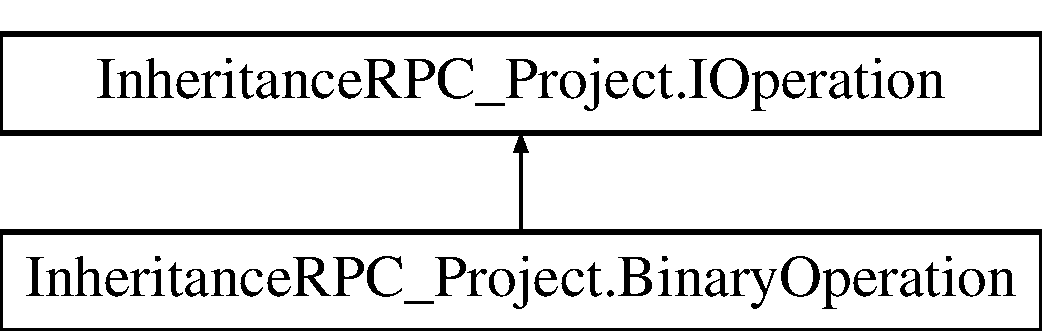
\includegraphics[height=2.000000cm]{class_inheritance_r_p_c___project_1_1_binary_operation}
\end{center}
\end{figure}
\subsection*{Public Member Functions}
\begin{DoxyCompactItemize}
\item 
\hyperlink{class_inheritance_r_p_c___project_1_1_binary_operation_aab4b197966243a385f884d045138c030}{Binary\+Operation} (Func$<$ double, double, double $>$ operation)
\begin{DoxyCompactList}\small\item\em The constructor of the operation, which is used to give the class the function which it will use in the execute method. \end{DoxyCompactList}\item 
double \hyperlink{class_inheritance_r_p_c___project_1_1_binary_operation_a9c344c45450b8496e1f6537b1a467a6c}{Execute} (double arg1, params double\mbox{[}$\,$\mbox{]} argn)
\begin{DoxyCompactList}\small\item\em The Execute method which will use the operation field of the class to calculate the output given the 2 input doubles. \end{DoxyCompactList}\end{DoxyCompactItemize}


\subsection{Detailed Description}
An operation class which extends the \hyperlink{interface_inheritance_r_p_c___project_1_1_i_operation}{I\+Operation} interface, and therefore has an execute method which takes doubles as parametre. The class is meant to handle binary operations (operations with 2 doubles as input). 



\subsection{Constructor \& Destructor Documentation}
\hypertarget{class_inheritance_r_p_c___project_1_1_binary_operation_aab4b197966243a385f884d045138c030}{\index{Inheritance\+R\+P\+C\+\_\+\+Project\+::\+Binary\+Operation@{Inheritance\+R\+P\+C\+\_\+\+Project\+::\+Binary\+Operation}!Binary\+Operation@{Binary\+Operation}}
\index{Binary\+Operation@{Binary\+Operation}!Inheritance\+R\+P\+C\+\_\+\+Project\+::\+Binary\+Operation@{Inheritance\+R\+P\+C\+\_\+\+Project\+::\+Binary\+Operation}}
\subsubsection[{Binary\+Operation}]{\setlength{\rightskip}{0pt plus 5cm}Inheritance\+R\+P\+C\+\_\+\+Project.\+Binary\+Operation.\+Binary\+Operation (
\begin{DoxyParamCaption}
\item[{Func$<$ double, double, double $>$}]{operation}
\end{DoxyParamCaption}
)}}\label{class_inheritance_r_p_c___project_1_1_binary_operation_aab4b197966243a385f884d045138c030}


The constructor of the operation, which is used to give the class the function which it will use in the execute method. 


\begin{DoxyParams}{Parameters}
{\em operation} & The operation wanted as a function(2 inputs 1 output)\\
\hline
\end{DoxyParams}


\subsection{Member Function Documentation}
\hypertarget{class_inheritance_r_p_c___project_1_1_binary_operation_a9c344c45450b8496e1f6537b1a467a6c}{\index{Inheritance\+R\+P\+C\+\_\+\+Project\+::\+Binary\+Operation@{Inheritance\+R\+P\+C\+\_\+\+Project\+::\+Binary\+Operation}!Execute@{Execute}}
\index{Execute@{Execute}!Inheritance\+R\+P\+C\+\_\+\+Project\+::\+Binary\+Operation@{Inheritance\+R\+P\+C\+\_\+\+Project\+::\+Binary\+Operation}}
\subsubsection[{Execute}]{\setlength{\rightskip}{0pt plus 5cm}double Inheritance\+R\+P\+C\+\_\+\+Project.\+Binary\+Operation.\+Execute (
\begin{DoxyParamCaption}
\item[{double}]{arg1, }
\item[{params double\mbox{[}$\,$\mbox{]}}]{argn}
\end{DoxyParamCaption}
)}}\label{class_inheritance_r_p_c___project_1_1_binary_operation_a9c344c45450b8496e1f6537b1a467a6c}


The Execute method which will use the operation field of the class to calculate the output given the 2 input doubles. 


\begin{DoxyParams}{Parameters}
{\em arg1} & The first double given\\
\hline
{\em argn} & A number of doubles in an array\\
\hline
\end{DoxyParams}
\begin{DoxyReturn}{Returns}
The result of the operation field given arg1 and argn\mbox{[}0\mbox{]}
\end{DoxyReturn}


Implements \hyperlink{interface_inheritance_r_p_c___project_1_1_i_operation}{Inheritance\+R\+P\+C\+\_\+\+Project.\+I\+Operation}.



The documentation for this class was generated from the following file\+:\begin{DoxyCompactItemize}
\item 
E\+:/\+User (\+E)/\+Programming (\+E)/\+B\+D\+S\+A-\/\+Exercises/\+B\+D\+S\+A2014/\+Inheritance\+R\+P\+C\+\_\+\+Project/Inheritance\+R\+P\+C.\+cs\end{DoxyCompactItemize}

\hypertarget{class_inheritance_r_p_c___project_1_1_inheritance_r_p_c}{\section{Inheritance\+R\+P\+C\+\_\+\+Project.\+Inheritance\+R\+P\+C Class Reference}
\label{class_inheritance_r_p_c___project_1_1_inheritance_r_p_c}\index{Inheritance\+R\+P\+C\+\_\+\+Project.\+Inheritance\+R\+P\+C@{Inheritance\+R\+P\+C\+\_\+\+Project.\+Inheritance\+R\+P\+C}}
}


The class takes a string as input, and if the string is in the format of a reverse Polish calculator expression, then it will calculate and return the result. Features Can handle the operators\+: +, -\/, $\ast$, /, sqrt, cos, sin, abs and pow ($^\wedge$) Can handle negative numbers if written in the form -\/x Can handle doubles if written in the form x,x Tokens are separated by a whitespace. If the input is invalid an exception is thrown. The class uses a dictionary$<$string, I\+Operation$>$ to handle the operations. To add an operation simply add it to the dictionary. The class currently has \hyperlink{interface_inheritance_r_p_c___project_1_1_i_operation}{I\+Operation} classes for unary and binary operations but tienary and so on can be added by creating an inner class which implements the \hyperlink{interface_inheritance_r_p_c___project_1_1_i_operation}{I\+Operation} interface.\+s  


\subsection*{Public Member Functions}
\begin{DoxyCompactItemize}
\item 
\hyperlink{class_inheritance_r_p_c___project_1_1_inheritance_r_p_c_ad34c70442f6f3696e800c3937f5bfd20}{Inheritance\+R\+P\+C} ()
\begin{DoxyCompactList}\small\item\em Constructor which sets up the class. \end{DoxyCompactList}\item 
double \hyperlink{class_inheritance_r_p_c___project_1_1_inheritance_r_p_c_a98c2f1992b820eba5b7528554c3c7d96}{Calculate\+Expression} (string rpce)
\begin{DoxyCompactList}\small\item\em Calculates the input reverse calculator string expression. Throws exceptions if the input is not in the R\+P\+C format. \end{DoxyCompactList}\end{DoxyCompactItemize}


\subsection{Detailed Description}
The class takes a string as input, and if the string is in the format of a reverse Polish calculator expression, then it will calculate and return the result. Features Can handle the operators\+: +, -\/, $\ast$, /, sqrt, cos, sin, abs and pow ($^\wedge$) Can handle negative numbers if written in the form -\/x Can handle doubles if written in the form x,x Tokens are separated by a whitespace. If the input is invalid an exception is thrown. The class uses a dictionary$<$string, I\+Operation$>$ to handle the operations. To add an operation simply add it to the dictionary. The class currently has \hyperlink{interface_inheritance_r_p_c___project_1_1_i_operation}{I\+Operation} classes for unary and binary operations but tienary and so on can be added by creating an inner class which implements the \hyperlink{interface_inheritance_r_p_c___project_1_1_i_operation}{I\+Operation} interface.\+s 



\subsection{Constructor \& Destructor Documentation}
\hypertarget{class_inheritance_r_p_c___project_1_1_inheritance_r_p_c_ad34c70442f6f3696e800c3937f5bfd20}{\index{Inheritance\+R\+P\+C\+\_\+\+Project\+::\+Inheritance\+R\+P\+C@{Inheritance\+R\+P\+C\+\_\+\+Project\+::\+Inheritance\+R\+P\+C}!Inheritance\+R\+P\+C@{Inheritance\+R\+P\+C}}
\index{Inheritance\+R\+P\+C@{Inheritance\+R\+P\+C}!Inheritance\+R\+P\+C\+\_\+\+Project\+::\+Inheritance\+R\+P\+C@{Inheritance\+R\+P\+C\+\_\+\+Project\+::\+Inheritance\+R\+P\+C}}
\subsubsection[{Inheritance\+R\+P\+C}]{\setlength{\rightskip}{0pt plus 5cm}Inheritance\+R\+P\+C\+\_\+\+Project.\+Inheritance\+R\+P\+C.\+Inheritance\+R\+P\+C (
\begin{DoxyParamCaption}
{}
\end{DoxyParamCaption}
)}}\label{class_inheritance_r_p_c___project_1_1_inheritance_r_p_c_ad34c70442f6f3696e800c3937f5bfd20}


Constructor which sets up the class. 



\subsection{Member Function Documentation}
\hypertarget{class_inheritance_r_p_c___project_1_1_inheritance_r_p_c_a98c2f1992b820eba5b7528554c3c7d96}{\index{Inheritance\+R\+P\+C\+\_\+\+Project\+::\+Inheritance\+R\+P\+C@{Inheritance\+R\+P\+C\+\_\+\+Project\+::\+Inheritance\+R\+P\+C}!Calculate\+Expression@{Calculate\+Expression}}
\index{Calculate\+Expression@{Calculate\+Expression}!Inheritance\+R\+P\+C\+\_\+\+Project\+::\+Inheritance\+R\+P\+C@{Inheritance\+R\+P\+C\+\_\+\+Project\+::\+Inheritance\+R\+P\+C}}
\subsubsection[{Calculate\+Expression}]{\setlength{\rightskip}{0pt plus 5cm}double Inheritance\+R\+P\+C\+\_\+\+Project.\+Inheritance\+R\+P\+C.\+Calculate\+Expression (
\begin{DoxyParamCaption}
\item[{string}]{rpce}
\end{DoxyParamCaption}
)}}\label{class_inheritance_r_p_c___project_1_1_inheritance_r_p_c_a98c2f1992b820eba5b7528554c3c7d96}


Calculates the input reverse calculator string expression. Throws exceptions if the input is not in the R\+P\+C format. 


\begin{DoxyParams}{Parameters}
{\em rpce} & A String in the Reverse Polish Calculator expression format\\
\hline
\end{DoxyParams}
\begin{DoxyReturn}{Returns}
0 if input is null or empty, otherwise returns the result
\end{DoxyReturn}


The documentation for this class was generated from the following file\+:\begin{DoxyCompactItemize}
\item 
E\+:/\+User (\+E)/\+Programming (\+E)/\+B\+D\+S\+A-\/\+Exercises/\+B\+D\+S\+A2014/\+Inheritance\+R\+P\+C\+\_\+\+Project/Inheritance\+R\+P\+C.\+cs\end{DoxyCompactItemize}

\hypertarget{class_inheritance_r_p_c___project_1_1_inheritance_r_p_ctests}{\section{Inheritance\+R\+P\+C\+\_\+\+Project.\+Inheritance\+R\+P\+Ctests Class Reference}
\label{class_inheritance_r_p_c___project_1_1_inheritance_r_p_ctests}\index{Inheritance\+R\+P\+C\+\_\+\+Project.\+Inheritance\+R\+P\+Ctests@{Inheritance\+R\+P\+C\+\_\+\+Project.\+Inheritance\+R\+P\+Ctests}}
}
\subsection*{Public Member Functions}
\begin{DoxyCompactItemize}
\item 
\hypertarget{class_inheritance_r_p_c___project_1_1_inheritance_r_p_ctests_ae9916e05afb98530099b931081a67a5d}{void {\bfseries Setup} ()}\label{class_inheritance_r_p_c___project_1_1_inheritance_r_p_ctests_ae9916e05afb98530099b931081a67a5d}

\item 
void \hyperlink{class_inheritance_r_p_c___project_1_1_inheritance_r_p_ctests_a4c6edd31f8ff287ac9a618596e5d8633}{Test\+Null\+Input} ()
\begin{DoxyCompactList}\small\item\em Testcase where the input is null -\/ should return 0. \end{DoxyCompactList}\item 
void \hyperlink{class_inheritance_r_p_c___project_1_1_inheritance_r_p_ctests_a40139282f6bc5a4363c8db540655dfb4}{Test\+Empty\+Input} ()
\begin{DoxyCompactList}\small\item\em Testcase where the input is \char`\"{}\char`\"{} -\/ should return 0. \end{DoxyCompactList}\item 
void \hyperlink{class_inheritance_r_p_c___project_1_1_inheritance_r_p_ctests_a32c3a70765db243c4ad0d53f9ea91d59}{Test\+Plus\+Operator} ()
\begin{DoxyCompactList}\small\item\em Testcase where the input contains a + operator (5 5 +) -\/ should return 10. \end{DoxyCompactList}\item 
void \hyperlink{class_inheritance_r_p_c___project_1_1_inheritance_r_p_ctests_a4634991cebc634f25d8877382142f1f8}{Test\+Minus\+Operator} ()
\begin{DoxyCompactList}\small\item\em Testcase where the input contains a -\/ operator (3 5 -\/) -\/ should return -\/2. \end{DoxyCompactList}\item 
void \hyperlink{class_inheritance_r_p_c___project_1_1_inheritance_r_p_ctests_a46d87cf2cd663bed9f7a26baab95391c}{Test\+Multiply\+Operator} ()
\begin{DoxyCompactList}\small\item\em Testcase where the input contains a $\ast$ operator (3 4 $\ast$) -\/ should return 12. \end{DoxyCompactList}\item 
void \hyperlink{class_inheritance_r_p_c___project_1_1_inheritance_r_p_ctests_a3ef7bd9323a34056c802c84825131468}{Test\+Divide\+Operator} ()
\begin{DoxyCompactList}\small\item\em Testcase where the input contains a / operator (12 4 $\ast$) -\/ should return 3. \end{DoxyCompactList}\item 
void \hyperlink{class_inheritance_r_p_c___project_1_1_inheritance_r_p_ctests_aa9c399d75f02fc273e271d580286a97b}{Test\+Pow\+Operator} ()
\begin{DoxyCompactList}\small\item\em Testcase where the input contains a pov ($^\wedge$) operator (5 2 pov) -\/ should return 25. (2 5 $^\wedge$) -\/ should return 32. \end{DoxyCompactList}\item 
void \hyperlink{class_inheritance_r_p_c___project_1_1_inheritance_r_p_ctests_a89d070a8b13358f0ab48bf1182609680}{Test\+Sin\+Operator} ()
\begin{DoxyCompactList}\small\item\em Testcase where the input contains sin operator (30 sin) -\/ should return Math.\+Sin(30). \end{DoxyCompactList}\item 
void \hyperlink{class_inheritance_r_p_c___project_1_1_inheritance_r_p_ctests_ae9bb58e3c9c18e96211ccb350f1b61e6}{Test\+Cos\+Operator} ()
\begin{DoxyCompactList}\small\item\em Testcase where the input contains cos operator (30 cos) -\/ should return Math.\+Cos(30). \end{DoxyCompactList}\item 
void \hyperlink{class_inheritance_r_p_c___project_1_1_inheritance_r_p_ctests_accf0b71829cd2bf549e23f582b177442}{Test\+Sqrt\+Operator} ()
\begin{DoxyCompactList}\small\item\em Testcase where the input contains sqrt operator (25 sqrt) -\/ should return Math.\+Cos(5). \end{DoxyCompactList}\item 
void \hyperlink{class_inheritance_r_p_c___project_1_1_inheritance_r_p_ctests_a552277330403bfd1df1089e8237a1f9e}{Test\+Abs\+Operator} ()
\begin{DoxyCompactList}\small\item\em Testcase where the input contains abs operator (25 abs, -\/25 abs, 0 abs, -\/0 abs) -\/ should return Math.\+Cos(5). \end{DoxyCompactList}\item 
void \hyperlink{class_inheritance_r_p_c___project_1_1_inheritance_r_p_ctests_ae1764b34b6a1bf3a16632c54c8959e23}{Test\+Complex\+Expression\+Operator} ()
\begin{DoxyCompactList}\small\item\em Testcase where the input contains multiple operators and values. \end{DoxyCompactList}\item 
void \hyperlink{class_inheritance_r_p_c___project_1_1_inheritance_r_p_ctests_a665b3473a8437f81c30d55ae8893fe8f}{Test\+Expression\+With\+Letters\+Operator} ()
\begin{DoxyCompactList}\small\item\em Testcase where the input contains letters and letters combined with numbers. \end{DoxyCompactList}\end{DoxyCompactItemize}


\subsection{Member Function Documentation}
\hypertarget{class_inheritance_r_p_c___project_1_1_inheritance_r_p_ctests_a552277330403bfd1df1089e8237a1f9e}{\index{Inheritance\+R\+P\+C\+\_\+\+Project\+::\+Inheritance\+R\+P\+Ctests@{Inheritance\+R\+P\+C\+\_\+\+Project\+::\+Inheritance\+R\+P\+Ctests}!Test\+Abs\+Operator@{Test\+Abs\+Operator}}
\index{Test\+Abs\+Operator@{Test\+Abs\+Operator}!Inheritance\+R\+P\+C\+\_\+\+Project\+::\+Inheritance\+R\+P\+Ctests@{Inheritance\+R\+P\+C\+\_\+\+Project\+::\+Inheritance\+R\+P\+Ctests}}
\subsubsection[{Test\+Abs\+Operator}]{\setlength{\rightskip}{0pt plus 5cm}void Inheritance\+R\+P\+C\+\_\+\+Project.\+Inheritance\+R\+P\+Ctests.\+Test\+Abs\+Operator (
\begin{DoxyParamCaption}
{}
\end{DoxyParamCaption}
)}}\label{class_inheritance_r_p_c___project_1_1_inheritance_r_p_ctests_a552277330403bfd1df1089e8237a1f9e}


Testcase where the input contains abs operator (25 abs, -\/25 abs, 0 abs, -\/0 abs) -\/ should return Math.\+Cos(5). 

\hypertarget{class_inheritance_r_p_c___project_1_1_inheritance_r_p_ctests_ae1764b34b6a1bf3a16632c54c8959e23}{\index{Inheritance\+R\+P\+C\+\_\+\+Project\+::\+Inheritance\+R\+P\+Ctests@{Inheritance\+R\+P\+C\+\_\+\+Project\+::\+Inheritance\+R\+P\+Ctests}!Test\+Complex\+Expression\+Operator@{Test\+Complex\+Expression\+Operator}}
\index{Test\+Complex\+Expression\+Operator@{Test\+Complex\+Expression\+Operator}!Inheritance\+R\+P\+C\+\_\+\+Project\+::\+Inheritance\+R\+P\+Ctests@{Inheritance\+R\+P\+C\+\_\+\+Project\+::\+Inheritance\+R\+P\+Ctests}}
\subsubsection[{Test\+Complex\+Expression\+Operator}]{\setlength{\rightskip}{0pt plus 5cm}void Inheritance\+R\+P\+C\+\_\+\+Project.\+Inheritance\+R\+P\+Ctests.\+Test\+Complex\+Expression\+Operator (
\begin{DoxyParamCaption}
{}
\end{DoxyParamCaption}
)}}\label{class_inheritance_r_p_c___project_1_1_inheritance_r_p_ctests_ae1764b34b6a1bf3a16632c54c8959e23}


Testcase where the input contains multiple operators and values. 

\hypertarget{class_inheritance_r_p_c___project_1_1_inheritance_r_p_ctests_ae9bb58e3c9c18e96211ccb350f1b61e6}{\index{Inheritance\+R\+P\+C\+\_\+\+Project\+::\+Inheritance\+R\+P\+Ctests@{Inheritance\+R\+P\+C\+\_\+\+Project\+::\+Inheritance\+R\+P\+Ctests}!Test\+Cos\+Operator@{Test\+Cos\+Operator}}
\index{Test\+Cos\+Operator@{Test\+Cos\+Operator}!Inheritance\+R\+P\+C\+\_\+\+Project\+::\+Inheritance\+R\+P\+Ctests@{Inheritance\+R\+P\+C\+\_\+\+Project\+::\+Inheritance\+R\+P\+Ctests}}
\subsubsection[{Test\+Cos\+Operator}]{\setlength{\rightskip}{0pt plus 5cm}void Inheritance\+R\+P\+C\+\_\+\+Project.\+Inheritance\+R\+P\+Ctests.\+Test\+Cos\+Operator (
\begin{DoxyParamCaption}
{}
\end{DoxyParamCaption}
)}}\label{class_inheritance_r_p_c___project_1_1_inheritance_r_p_ctests_ae9bb58e3c9c18e96211ccb350f1b61e6}


Testcase where the input contains cos operator (30 cos) -\/ should return Math.\+Cos(30). 

\hypertarget{class_inheritance_r_p_c___project_1_1_inheritance_r_p_ctests_a3ef7bd9323a34056c802c84825131468}{\index{Inheritance\+R\+P\+C\+\_\+\+Project\+::\+Inheritance\+R\+P\+Ctests@{Inheritance\+R\+P\+C\+\_\+\+Project\+::\+Inheritance\+R\+P\+Ctests}!Test\+Divide\+Operator@{Test\+Divide\+Operator}}
\index{Test\+Divide\+Operator@{Test\+Divide\+Operator}!Inheritance\+R\+P\+C\+\_\+\+Project\+::\+Inheritance\+R\+P\+Ctests@{Inheritance\+R\+P\+C\+\_\+\+Project\+::\+Inheritance\+R\+P\+Ctests}}
\subsubsection[{Test\+Divide\+Operator}]{\setlength{\rightskip}{0pt plus 5cm}void Inheritance\+R\+P\+C\+\_\+\+Project.\+Inheritance\+R\+P\+Ctests.\+Test\+Divide\+Operator (
\begin{DoxyParamCaption}
{}
\end{DoxyParamCaption}
)}}\label{class_inheritance_r_p_c___project_1_1_inheritance_r_p_ctests_a3ef7bd9323a34056c802c84825131468}


Testcase where the input contains a / operator (12 4 $\ast$) -\/ should return 3. 

\hypertarget{class_inheritance_r_p_c___project_1_1_inheritance_r_p_ctests_a40139282f6bc5a4363c8db540655dfb4}{\index{Inheritance\+R\+P\+C\+\_\+\+Project\+::\+Inheritance\+R\+P\+Ctests@{Inheritance\+R\+P\+C\+\_\+\+Project\+::\+Inheritance\+R\+P\+Ctests}!Test\+Empty\+Input@{Test\+Empty\+Input}}
\index{Test\+Empty\+Input@{Test\+Empty\+Input}!Inheritance\+R\+P\+C\+\_\+\+Project\+::\+Inheritance\+R\+P\+Ctests@{Inheritance\+R\+P\+C\+\_\+\+Project\+::\+Inheritance\+R\+P\+Ctests}}
\subsubsection[{Test\+Empty\+Input}]{\setlength{\rightskip}{0pt plus 5cm}void Inheritance\+R\+P\+C\+\_\+\+Project.\+Inheritance\+R\+P\+Ctests.\+Test\+Empty\+Input (
\begin{DoxyParamCaption}
{}
\end{DoxyParamCaption}
)}}\label{class_inheritance_r_p_c___project_1_1_inheritance_r_p_ctests_a40139282f6bc5a4363c8db540655dfb4}


Testcase where the input is \char`\"{}\char`\"{} -\/ should return 0. 

\hypertarget{class_inheritance_r_p_c___project_1_1_inheritance_r_p_ctests_a665b3473a8437f81c30d55ae8893fe8f}{\index{Inheritance\+R\+P\+C\+\_\+\+Project\+::\+Inheritance\+R\+P\+Ctests@{Inheritance\+R\+P\+C\+\_\+\+Project\+::\+Inheritance\+R\+P\+Ctests}!Test\+Expression\+With\+Letters\+Operator@{Test\+Expression\+With\+Letters\+Operator}}
\index{Test\+Expression\+With\+Letters\+Operator@{Test\+Expression\+With\+Letters\+Operator}!Inheritance\+R\+P\+C\+\_\+\+Project\+::\+Inheritance\+R\+P\+Ctests@{Inheritance\+R\+P\+C\+\_\+\+Project\+::\+Inheritance\+R\+P\+Ctests}}
\subsubsection[{Test\+Expression\+With\+Letters\+Operator}]{\setlength{\rightskip}{0pt plus 5cm}void Inheritance\+R\+P\+C\+\_\+\+Project.\+Inheritance\+R\+P\+Ctests.\+Test\+Expression\+With\+Letters\+Operator (
\begin{DoxyParamCaption}
{}
\end{DoxyParamCaption}
)}}\label{class_inheritance_r_p_c___project_1_1_inheritance_r_p_ctests_a665b3473a8437f81c30d55ae8893fe8f}


Testcase where the input contains letters and letters combined with numbers. 

\hypertarget{class_inheritance_r_p_c___project_1_1_inheritance_r_p_ctests_a4634991cebc634f25d8877382142f1f8}{\index{Inheritance\+R\+P\+C\+\_\+\+Project\+::\+Inheritance\+R\+P\+Ctests@{Inheritance\+R\+P\+C\+\_\+\+Project\+::\+Inheritance\+R\+P\+Ctests}!Test\+Minus\+Operator@{Test\+Minus\+Operator}}
\index{Test\+Minus\+Operator@{Test\+Minus\+Operator}!Inheritance\+R\+P\+C\+\_\+\+Project\+::\+Inheritance\+R\+P\+Ctests@{Inheritance\+R\+P\+C\+\_\+\+Project\+::\+Inheritance\+R\+P\+Ctests}}
\subsubsection[{Test\+Minus\+Operator}]{\setlength{\rightskip}{0pt plus 5cm}void Inheritance\+R\+P\+C\+\_\+\+Project.\+Inheritance\+R\+P\+Ctests.\+Test\+Minus\+Operator (
\begin{DoxyParamCaption}
{}
\end{DoxyParamCaption}
)}}\label{class_inheritance_r_p_c___project_1_1_inheritance_r_p_ctests_a4634991cebc634f25d8877382142f1f8}


Testcase where the input contains a -\/ operator (3 5 -\/) -\/ should return -\/2. 

\hypertarget{class_inheritance_r_p_c___project_1_1_inheritance_r_p_ctests_a46d87cf2cd663bed9f7a26baab95391c}{\index{Inheritance\+R\+P\+C\+\_\+\+Project\+::\+Inheritance\+R\+P\+Ctests@{Inheritance\+R\+P\+C\+\_\+\+Project\+::\+Inheritance\+R\+P\+Ctests}!Test\+Multiply\+Operator@{Test\+Multiply\+Operator}}
\index{Test\+Multiply\+Operator@{Test\+Multiply\+Operator}!Inheritance\+R\+P\+C\+\_\+\+Project\+::\+Inheritance\+R\+P\+Ctests@{Inheritance\+R\+P\+C\+\_\+\+Project\+::\+Inheritance\+R\+P\+Ctests}}
\subsubsection[{Test\+Multiply\+Operator}]{\setlength{\rightskip}{0pt plus 5cm}void Inheritance\+R\+P\+C\+\_\+\+Project.\+Inheritance\+R\+P\+Ctests.\+Test\+Multiply\+Operator (
\begin{DoxyParamCaption}
{}
\end{DoxyParamCaption}
)}}\label{class_inheritance_r_p_c___project_1_1_inheritance_r_p_ctests_a46d87cf2cd663bed9f7a26baab95391c}


Testcase where the input contains a $\ast$ operator (3 4 $\ast$) -\/ should return 12. 

\hypertarget{class_inheritance_r_p_c___project_1_1_inheritance_r_p_ctests_a4c6edd31f8ff287ac9a618596e5d8633}{\index{Inheritance\+R\+P\+C\+\_\+\+Project\+::\+Inheritance\+R\+P\+Ctests@{Inheritance\+R\+P\+C\+\_\+\+Project\+::\+Inheritance\+R\+P\+Ctests}!Test\+Null\+Input@{Test\+Null\+Input}}
\index{Test\+Null\+Input@{Test\+Null\+Input}!Inheritance\+R\+P\+C\+\_\+\+Project\+::\+Inheritance\+R\+P\+Ctests@{Inheritance\+R\+P\+C\+\_\+\+Project\+::\+Inheritance\+R\+P\+Ctests}}
\subsubsection[{Test\+Null\+Input}]{\setlength{\rightskip}{0pt plus 5cm}void Inheritance\+R\+P\+C\+\_\+\+Project.\+Inheritance\+R\+P\+Ctests.\+Test\+Null\+Input (
\begin{DoxyParamCaption}
{}
\end{DoxyParamCaption}
)}}\label{class_inheritance_r_p_c___project_1_1_inheritance_r_p_ctests_a4c6edd31f8ff287ac9a618596e5d8633}


Testcase where the input is null -\/ should return 0. 

\hypertarget{class_inheritance_r_p_c___project_1_1_inheritance_r_p_ctests_a32c3a70765db243c4ad0d53f9ea91d59}{\index{Inheritance\+R\+P\+C\+\_\+\+Project\+::\+Inheritance\+R\+P\+Ctests@{Inheritance\+R\+P\+C\+\_\+\+Project\+::\+Inheritance\+R\+P\+Ctests}!Test\+Plus\+Operator@{Test\+Plus\+Operator}}
\index{Test\+Plus\+Operator@{Test\+Plus\+Operator}!Inheritance\+R\+P\+C\+\_\+\+Project\+::\+Inheritance\+R\+P\+Ctests@{Inheritance\+R\+P\+C\+\_\+\+Project\+::\+Inheritance\+R\+P\+Ctests}}
\subsubsection[{Test\+Plus\+Operator}]{\setlength{\rightskip}{0pt plus 5cm}void Inheritance\+R\+P\+C\+\_\+\+Project.\+Inheritance\+R\+P\+Ctests.\+Test\+Plus\+Operator (
\begin{DoxyParamCaption}
{}
\end{DoxyParamCaption}
)}}\label{class_inheritance_r_p_c___project_1_1_inheritance_r_p_ctests_a32c3a70765db243c4ad0d53f9ea91d59}


Testcase where the input contains a + operator (5 5 +) -\/ should return 10. 

\hypertarget{class_inheritance_r_p_c___project_1_1_inheritance_r_p_ctests_aa9c399d75f02fc273e271d580286a97b}{\index{Inheritance\+R\+P\+C\+\_\+\+Project\+::\+Inheritance\+R\+P\+Ctests@{Inheritance\+R\+P\+C\+\_\+\+Project\+::\+Inheritance\+R\+P\+Ctests}!Test\+Pow\+Operator@{Test\+Pow\+Operator}}
\index{Test\+Pow\+Operator@{Test\+Pow\+Operator}!Inheritance\+R\+P\+C\+\_\+\+Project\+::\+Inheritance\+R\+P\+Ctests@{Inheritance\+R\+P\+C\+\_\+\+Project\+::\+Inheritance\+R\+P\+Ctests}}
\subsubsection[{Test\+Pow\+Operator}]{\setlength{\rightskip}{0pt plus 5cm}void Inheritance\+R\+P\+C\+\_\+\+Project.\+Inheritance\+R\+P\+Ctests.\+Test\+Pow\+Operator (
\begin{DoxyParamCaption}
{}
\end{DoxyParamCaption}
)}}\label{class_inheritance_r_p_c___project_1_1_inheritance_r_p_ctests_aa9c399d75f02fc273e271d580286a97b}


Testcase where the input contains a pov ($^\wedge$) operator (5 2 pov) -\/ should return 25. (2 5 $^\wedge$) -\/ should return 32. 

\hypertarget{class_inheritance_r_p_c___project_1_1_inheritance_r_p_ctests_a89d070a8b13358f0ab48bf1182609680}{\index{Inheritance\+R\+P\+C\+\_\+\+Project\+::\+Inheritance\+R\+P\+Ctests@{Inheritance\+R\+P\+C\+\_\+\+Project\+::\+Inheritance\+R\+P\+Ctests}!Test\+Sin\+Operator@{Test\+Sin\+Operator}}
\index{Test\+Sin\+Operator@{Test\+Sin\+Operator}!Inheritance\+R\+P\+C\+\_\+\+Project\+::\+Inheritance\+R\+P\+Ctests@{Inheritance\+R\+P\+C\+\_\+\+Project\+::\+Inheritance\+R\+P\+Ctests}}
\subsubsection[{Test\+Sin\+Operator}]{\setlength{\rightskip}{0pt plus 5cm}void Inheritance\+R\+P\+C\+\_\+\+Project.\+Inheritance\+R\+P\+Ctests.\+Test\+Sin\+Operator (
\begin{DoxyParamCaption}
{}
\end{DoxyParamCaption}
)}}\label{class_inheritance_r_p_c___project_1_1_inheritance_r_p_ctests_a89d070a8b13358f0ab48bf1182609680}


Testcase where the input contains sin operator (30 sin) -\/ should return Math.\+Sin(30). 

\hypertarget{class_inheritance_r_p_c___project_1_1_inheritance_r_p_ctests_accf0b71829cd2bf549e23f582b177442}{\index{Inheritance\+R\+P\+C\+\_\+\+Project\+::\+Inheritance\+R\+P\+Ctests@{Inheritance\+R\+P\+C\+\_\+\+Project\+::\+Inheritance\+R\+P\+Ctests}!Test\+Sqrt\+Operator@{Test\+Sqrt\+Operator}}
\index{Test\+Sqrt\+Operator@{Test\+Sqrt\+Operator}!Inheritance\+R\+P\+C\+\_\+\+Project\+::\+Inheritance\+R\+P\+Ctests@{Inheritance\+R\+P\+C\+\_\+\+Project\+::\+Inheritance\+R\+P\+Ctests}}
\subsubsection[{Test\+Sqrt\+Operator}]{\setlength{\rightskip}{0pt plus 5cm}void Inheritance\+R\+P\+C\+\_\+\+Project.\+Inheritance\+R\+P\+Ctests.\+Test\+Sqrt\+Operator (
\begin{DoxyParamCaption}
{}
\end{DoxyParamCaption}
)}}\label{class_inheritance_r_p_c___project_1_1_inheritance_r_p_ctests_accf0b71829cd2bf549e23f582b177442}


Testcase where the input contains sqrt operator (25 sqrt) -\/ should return Math.\+Cos(5). 



The documentation for this class was generated from the following file\+:\begin{DoxyCompactItemize}
\item 
E\+:/\+User (\+E)/\+Programming (\+E)/\+B\+D\+S\+A-\/\+Exercises/\+B\+D\+S\+A2014/\+Inheritance\+R\+P\+C\+\_\+\+Project/Inheritance\+R\+P\+C.\+tests.\+cs\end{DoxyCompactItemize}

\hypertarget{interface_inheritance_r_p_c___project_1_1_i_operation}{\section{Inheritance\+R\+P\+C\+\_\+\+Project.\+I\+Operation Interface Reference}
\label{interface_inheritance_r_p_c___project_1_1_i_operation}\index{Inheritance\+R\+P\+C\+\_\+\+Project.\+I\+Operation@{Inheritance\+R\+P\+C\+\_\+\+Project.\+I\+Operation}}
}


An interface which has an execute method which can take doubles as parametres.  


Inheritance diagram for Inheritance\+R\+P\+C\+\_\+\+Project.\+I\+Operation\+:\begin{figure}[H]
\begin{center}
\leavevmode
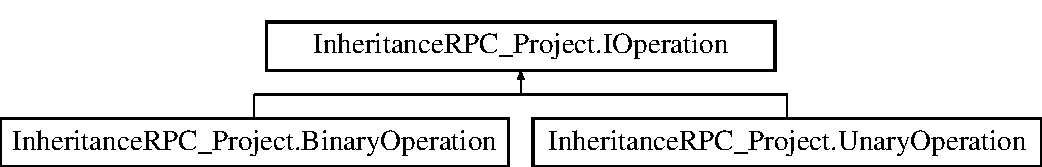
\includegraphics[height=2.000000cm]{interface_inheritance_r_p_c___project_1_1_i_operation}
\end{center}
\end{figure}
\subsection*{Public Member Functions}
\begin{DoxyCompactItemize}
\item 
\hypertarget{interface_inheritance_r_p_c___project_1_1_i_operation_abcab2f8bc2367a44c05e5244a1fea4eb}{double {\bfseries Execute} (double arg1, params double\mbox{[}$\,$\mbox{]} argn)}\label{interface_inheritance_r_p_c___project_1_1_i_operation_abcab2f8bc2367a44c05e5244a1fea4eb}

\end{DoxyCompactItemize}


\subsection{Detailed Description}
An interface which has an execute method which can take doubles as parametres. 



The documentation for this interface was generated from the following file\+:\begin{DoxyCompactItemize}
\item 
E\+:/\+User (\+E)/\+Programming (\+E)/\+B\+D\+S\+A-\/\+Exercises/\+B\+D\+S\+A2014/\+Inheritance\+R\+P\+C\+\_\+\+Project/Inheritance\+R\+P\+C.\+cs\end{DoxyCompactItemize}

\hypertarget{class_inheritance_r_p_c___project_1_1_unary_operation}{\section{Inheritance\+R\+P\+C\+\_\+\+Project.\+Unary\+Operation Class Reference}
\label{class_inheritance_r_p_c___project_1_1_unary_operation}\index{Inheritance\+R\+P\+C\+\_\+\+Project.\+Unary\+Operation@{Inheritance\+R\+P\+C\+\_\+\+Project.\+Unary\+Operation}}
}


An operation class which extends the \hyperlink{interface_inheritance_r_p_c___project_1_1_i_operation}{I\+Operation} interface, and therefore has an execute method which takes doubles as parametre. The class is meant to handle unary operations (operations with 1 double as input).  


Inheritance diagram for Inheritance\+R\+P\+C\+\_\+\+Project.\+Unary\+Operation\+:\begin{figure}[H]
\begin{center}
\leavevmode
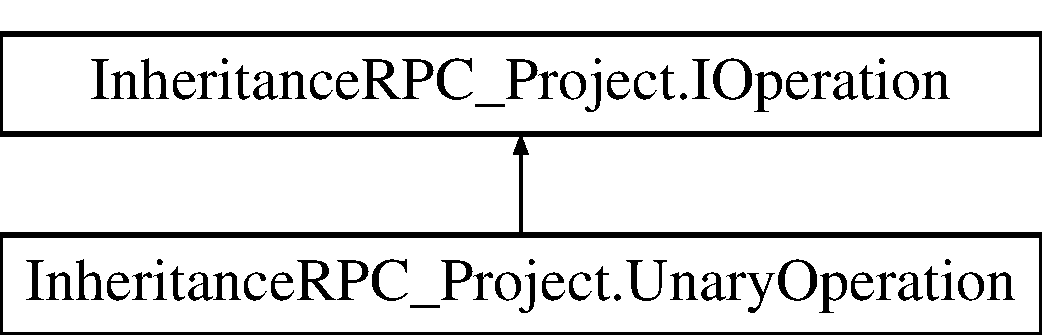
\includegraphics[height=2.000000cm]{class_inheritance_r_p_c___project_1_1_unary_operation}
\end{center}
\end{figure}
\subsection*{Public Member Functions}
\begin{DoxyCompactItemize}
\item 
\hyperlink{class_inheritance_r_p_c___project_1_1_unary_operation_abc91765e8e1775675d6b9f12747ad056}{Unary\+Operation} (Func$<$ double, double $>$ operation)
\begin{DoxyCompactList}\small\item\em The constructor of the operation, which is used to give the class the function which it will use in the execute method. \end{DoxyCompactList}\item 
double \hyperlink{class_inheritance_r_p_c___project_1_1_unary_operation_af5f32626af010e981e3e08aab753a61c}{Execute} (double arg1, params double\mbox{[}$\,$\mbox{]} argn)
\begin{DoxyCompactList}\small\item\em The Execute method which will use the operation field of the class to calculate the output given the input double. \end{DoxyCompactList}\end{DoxyCompactItemize}


\subsection{Detailed Description}
An operation class which extends the \hyperlink{interface_inheritance_r_p_c___project_1_1_i_operation}{I\+Operation} interface, and therefore has an execute method which takes doubles as parametre. The class is meant to handle unary operations (operations with 1 double as input). 



\subsection{Constructor \& Destructor Documentation}
\hypertarget{class_inheritance_r_p_c___project_1_1_unary_operation_abc91765e8e1775675d6b9f12747ad056}{\index{Inheritance\+R\+P\+C\+\_\+\+Project\+::\+Unary\+Operation@{Inheritance\+R\+P\+C\+\_\+\+Project\+::\+Unary\+Operation}!Unary\+Operation@{Unary\+Operation}}
\index{Unary\+Operation@{Unary\+Operation}!Inheritance\+R\+P\+C\+\_\+\+Project\+::\+Unary\+Operation@{Inheritance\+R\+P\+C\+\_\+\+Project\+::\+Unary\+Operation}}
\subsubsection[{Unary\+Operation}]{\setlength{\rightskip}{0pt plus 5cm}Inheritance\+R\+P\+C\+\_\+\+Project.\+Unary\+Operation.\+Unary\+Operation (
\begin{DoxyParamCaption}
\item[{Func$<$ double, double $>$}]{operation}
\end{DoxyParamCaption}
)}}\label{class_inheritance_r_p_c___project_1_1_unary_operation_abc91765e8e1775675d6b9f12747ad056}


The constructor of the operation, which is used to give the class the function which it will use in the execute method. 


\begin{DoxyParams}{Parameters}
{\em operation} & The operation wanted as a function(1 input 1 output)\\
\hline
\end{DoxyParams}


\subsection{Member Function Documentation}
\hypertarget{class_inheritance_r_p_c___project_1_1_unary_operation_af5f32626af010e981e3e08aab753a61c}{\index{Inheritance\+R\+P\+C\+\_\+\+Project\+::\+Unary\+Operation@{Inheritance\+R\+P\+C\+\_\+\+Project\+::\+Unary\+Operation}!Execute@{Execute}}
\index{Execute@{Execute}!Inheritance\+R\+P\+C\+\_\+\+Project\+::\+Unary\+Operation@{Inheritance\+R\+P\+C\+\_\+\+Project\+::\+Unary\+Operation}}
\subsubsection[{Execute}]{\setlength{\rightskip}{0pt plus 5cm}double Inheritance\+R\+P\+C\+\_\+\+Project.\+Unary\+Operation.\+Execute (
\begin{DoxyParamCaption}
\item[{double}]{arg1, }
\item[{params double\mbox{[}$\,$\mbox{]}}]{argn}
\end{DoxyParamCaption}
)}}\label{class_inheritance_r_p_c___project_1_1_unary_operation_af5f32626af010e981e3e08aab753a61c}


The Execute method which will use the operation field of the class to calculate the output given the input double. 


\begin{DoxyParams}{Parameters}
{\em arg1} & The first double given\\
\hline
{\em argn} & A number of doubles in an array\\
\hline
\end{DoxyParams}
\begin{DoxyReturn}{Returns}
The result of the operation field given arg1
\end{DoxyReturn}


Implements \hyperlink{interface_inheritance_r_p_c___project_1_1_i_operation}{Inheritance\+R\+P\+C\+\_\+\+Project.\+I\+Operation}.



The documentation for this class was generated from the following file\+:\begin{DoxyCompactItemize}
\item 
E\+:/\+User (\+E)/\+Programming (\+E)/\+B\+D\+S\+A-\/\+Exercises/\+B\+D\+S\+A2014/\+Inheritance\+R\+P\+C\+\_\+\+Project/Inheritance\+R\+P\+C.\+cs\end{DoxyCompactItemize}

%--- End generated contents ---

% Index
\newpage
\phantomsection
\addcontentsline{toc}{chapter}{Index}
\printindex

\end{document}
